\documentclass{article}
\usepackage[a4paper, margin=1in]{geometry}
\usepackage{amsmath}
\usepackage{graphicx}
\usepackage{hyperref}

\title{Time Series Forecasting of Appliance Energy Usage}
\author{Angel Diaz Carral}
\date{\today}

\begin{document}

\maketitle

\section{Introduction}

This project focuses on forecasting energy consumption using multivariate time series data. It demonstrates both deterministic and probabilistic deep learning approaches and highlights the benefits of modeling uncertainty in forecasting tasks.

\vspace{0.5em}
\noindent\textbf{Deliverables submitted:}
\begin{itemize}
  \item \textbf{Report:} This PDF document explaining the dataset, models, methodology, and conclusions.
  \item \textbf{Jupyter Notebooks:} A modular pipeline with three standalone notebooks:
  \begin{enumerate}
    \item \texttt{1\_eda.ipynb} Exploratory Data Analysis.
    \item \texttt{2\_training.ipynb} Training scripts for LSTM-VAE.
    \item \texttt{3\_evaluation.ipynb} Evaluation and visualization of results.
  \end{enumerate}
  \item \textbf{Python Package:} A production-ready package that includes:
  \begin{itemize}
    \item Trained model (\texttt{model.pkl})
    \item Inference and evaluation utilities
  \end{itemize}
  \item \textbf{GitHub Repository:} The full source code, notebooks, Dockerfile, and documentation can be found at:
  \begin{center}
    \texttt{\url{https://github.com/adiazcarral/ADC-TestDataScience-2}}
  \end{center}
\end{itemize}

\vspace{0.5em}
The following sections explain the methodology, data preprocessing, model training, and key insights derived from this work.

\section{Dataset}
The dataset consists of multivariate sensor readings recorded every 10 minutes from a household. It includes 28 input variables (e.g., lights, temperature, humidity) and one target variable: \texttt{Appliances}, representing the energy consumed.

\section{Exploratory Data Analysis (EDA)}

In the EDA notebook (\texttt{01\_eda.ipynb}), we begin by analyzing the data's key features, understanding the distribution of variables, and identifying any patterns, missing values, or outliers. The focus is on gaining insights into the temporal behavior of the dataset, especially the energy consumption patterns.

\begin{figure}[h!]
    \centering
    \includegraphics[width=1.0\textwidth]{pics/Appliances.png}
    \caption{Visualization of target "Appliances"}
\end{figure}

\subsection{Seasonality Analysis}
One of the key components of the exploratory analysis is the study of seasonality in the energy consumption data. To detect seasonality, I performed the following tests and analyses:

\begin{itemize}
  \item \textbf{Seasonal Decomposition of Time Series (STL):} The dataset was decomposed using STL decomposition to separate the time series into trend, seasonal, and residual components. This helped identify any repeating patterns in energy usage over different periods, such as daily or seasonal cycles.
  \item \textbf{Autocorrelation Function (ACF):} I plotted the ACF to identify periodic correlations in the data. Peaks in the ACF plot at specific lags indicate seasonality at those intervals (e.g., daily, weekly, yearly).
  \item \textbf{Fourier Transform:} A Fourier Transform was applied to the data to examine the dominant frequencies in the time series. Significant peaks in the frequency domain suggest the presence of seasonal cycles.
  \item \textbf{Heatmaps of Hourly and Daily Energy Consumption:} Heatmaps were created to visualize the variation in energy usage across different hours of the day and days of the week, further helping to confirm any seasonal patterns.
\end{itemize}

These methods provided a comprehensive understanding of the seasonal variations in energy consumption, allowing for better modeling decisions when handling time series forecasts.

\subsection{Data Preprocessing}
After studying seasonality, the data was cleaned and preprocessed to address any missing values, scaling issues, and potential outliers. A filter was applied to remove any blurry or unclear observations that could negatively impact model performance.
\section{Forecasting Models}
We compare two deep learning architectures:

\subsection{RNN (Deterministic)}
A classic recurrent neural network trained to produce point forecasts. It is simple, efficient, and suitable for baseline performance.

\subsection{LSTM-VAE (Probabilistic)}
The LSTM-VAE model is an enhanced version of the variational autoencoder (VAE) architecture, adapted for time series forecasting. This model combines an LSTM-based encoder-decoder framework with the probabilistic nature of a VAE to generate probabilistic forecasts.

\textbf{Architecture:}
The model operates in a sequence-to-one (seq2one) setup, where a sequence of past observations is encoded into a latent space, which is then decoded to predict the future. The key components are:

\begin{itemize}
  \item \textbf{Encoder:} The LSTM-based encoder processes the input sequence (100 time steps) and compresses the temporal information into a probabilistic latent space, represented by a mean and variance (from a Gaussian distribution).
  \item \textbf{Latent Space:} The latent space encodes the underlying dynamics of the time series, capturing the temporal correlations in the data. By sampling from this latent space, we can model uncertainty in the forecast.
  \item \textbf{Decoder:} The decoder takes the sampled latent variable and generates the predicted future values (100 time steps of the \texttt{Appliances} variable).
  \item \textbf{Probabilistic Forecasting:} The model outputs both the predicted mean and uncertainty intervals for each time step, providing a range of possible future scenarios rather than a single point forecast.
\end{itemize}

\textbf{Training:}
The LSTM-VAE model is trained by minimizing the combination of the reconstruction loss (measuring the difference between the predicted and actual future values) and the Kullback-Leibler (KL) divergence (penalizing the difference between the learned latent distribution and the prior). This approach ensures the latent space is structured and the model can generalize well to unseen data.

\textbf{Advantages:}
\begin{itemize}
  \item Captures temporal dependencies in the data through the LSTM architecture.
  \item Provides probabilistic forecasts, offering uncertainty estimates for future predictions.
  \item More robust to noisy or missing data, as it learns to generate plausible future values by sampling from the learned distribution.
\end{itemize}

\section{Training Setup}
\textbf{Input-output windows:} Each training sample consists of:
\begin{itemize}
  \item \textbf{Input ($X$):} A sequence of historical multivariate sensor readings of length \texttt{input\_window} (e.g., 100), \textbf{taken from the past}. To avoid data leakage, we introduce a \textbf{forecast horizon} — a gap between the end of the input and the prediction target. For instance, to predict $y_{t+1}$, the model receives input from $[t - 199, \dots, t - 100]$ — that is, the model learns to forecast values 100 steps ahead using earlier data.
  \item \textbf{Target ($y$):} The "Appliances" value at time step $t + 1$.
\end{itemize}

This results in a forecasting task with a fixed \textbf{lead time of 100 steps}, mimicking real-world scenarios where decisions must be made in advance without access to future measurements.

We explore two training regimes:
\begin{itemize}
  \item \textbf{Direct forecasting:} Predict all 100 steps in a single forward pass.
  \item \textbf{One-step forecasting:} Predict one step at a time recursively.
\end{itemize}

\section{Validation and Evaluation}

We compare the performance of the models in two settings: direct forecasting and one-step autoregressive forecasting. The following figures illustrate the results for each of these two approaches. We split the data into training, validation, and test sets. Evaluation metrics (jupyter notebook 03) include:
\begin{itemize}
  \item MAE (Mean Absolute Error)
  \item RMSE (Root Mean Squared Error)
  \item $R^2$ score
  \item CRPS (Continuous Ranked Probability Score) for probabilistic models
\end{itemize}

\subsection{Direct Forecasting}
In direct forecasting, the model predicts all 100 steps in one forward pass. This approach evaluates the model's ability to make long-term predictions in a single step.

\begin{figure}[h!]
    \centering
    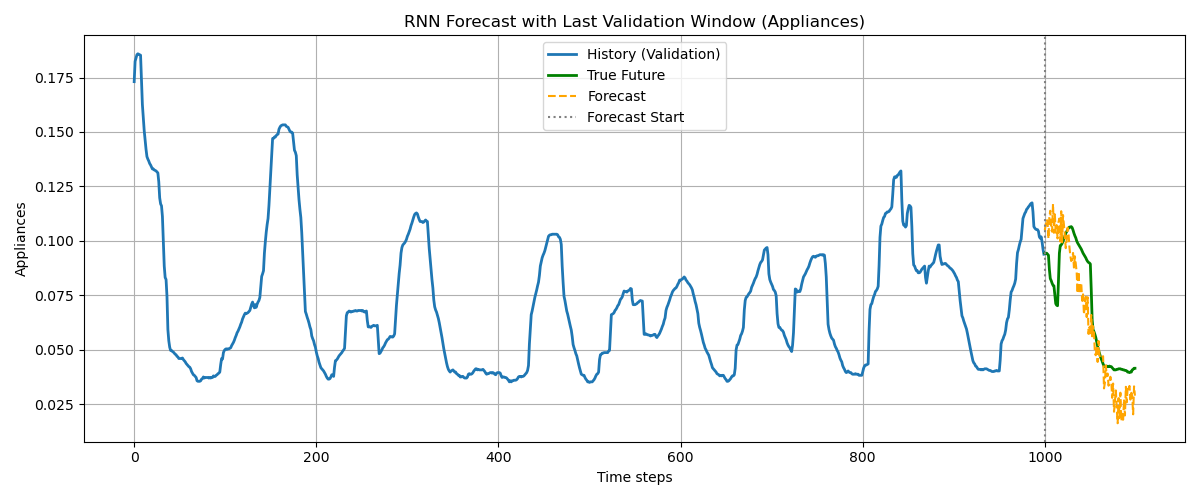
\includegraphics[width=1\textwidth]{pics/rnn_direct_forecast.png}
    \caption{Performance comparison of RNN on the validation set for one-step forecasting.}
    \label{fig:one_step_forecasting_comparison}
\end{figure}

\begin{figure}[h!]
    \centering
    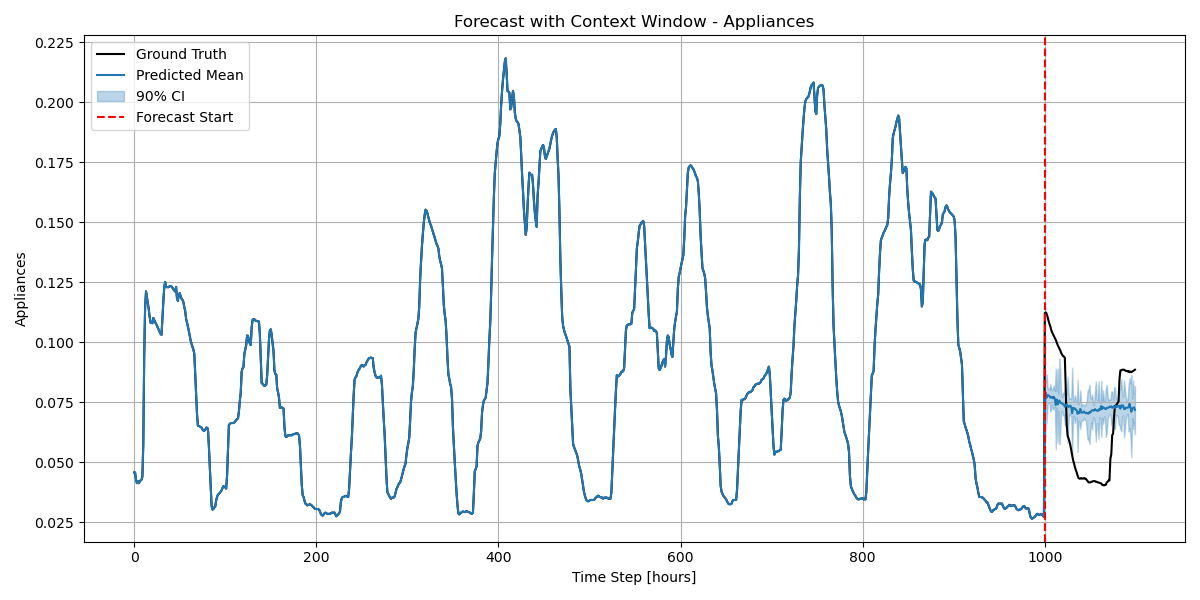
\includegraphics[width=1\textwidth]{pics/lstmvae_direct_forecast.png}
    \caption{Performance comparison of LSTM-VAE on the validation set for one-step forecasting.}
    \label{fig:one_step_forecasting_error}
\end{figure}

\subsection{One-Step Forecasting}
In the one-step forecasting approach, the model predicts one step at a time. This method is generally slower but may offer better performance for certain time series tasks.

\begin{figure}[h!]
    \centering
    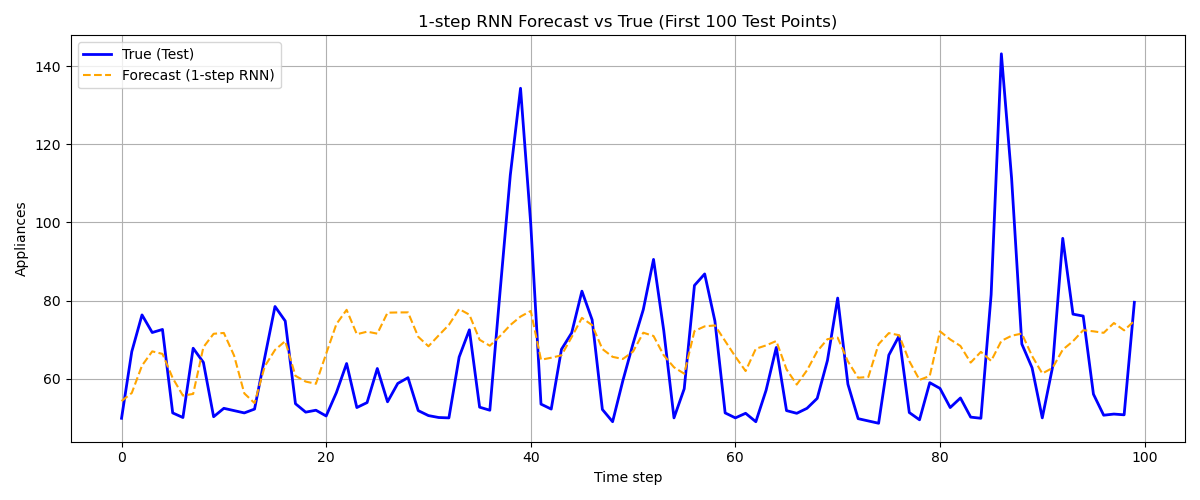
\includegraphics[width=1\textwidth]{pics/rnn1step.png}
    \caption{Performance comparison of RNN on the validation set for direct forecasting.}
    \label{fig:direct_forecasting_comparison}
\end{figure}

\begin{figure}[h!]
    \centering
    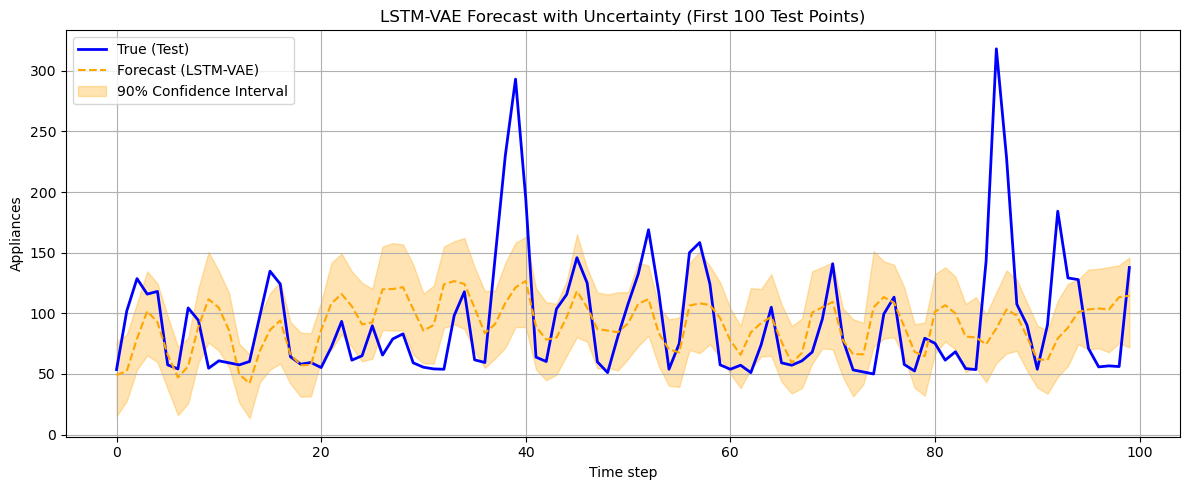
\includegraphics[width=1\textwidth]{pics/lstm1step.png}
    \caption{Performance comparison of LSTM-VAE on the validation set for direct forecasting.}
    \label{fig:direct_forecasting_error}
\end{figure}

The \textbf{LSTM-VAE} consistently provides more stable predictions with tighter confidence intervals and competitive RMSE/MAE, making it favorable for deployment.

\section{Conclusions}
The probabilistic approach using an LSTM-VAE offers significant advantages:
\begin{itemize}
  \item Captures uncertainty in long-term forecasts.
  \item Produces more informative predictions (intervals, distributions).
  \item Robust to noisy or incomplete data.
\end{itemize}

Adapting an image-focused architecture (VAE) to time series required careful reshaping of data and replacing convolutional layers with LSTM cells. This allowed the latent representation to encode temporal dynamics rather than spatial patterns.

\section{Final Remarks}
Probabilistic forecasting is essential in energy modeling and many real-world domains where uncertainty matters. This project demonstrates how modern deep generative models can be adapted and applied effectively to sequential problems.

\end{document}